\documentclass[]{article}
\usepackage{lmodern}
\usepackage{amssymb,amsmath}
\usepackage{ifxetex,ifluatex}
\usepackage{fixltx2e} % provides \textsubscript
\ifnum 0\ifxetex 1\fi\ifluatex 1\fi=0 % if pdftex
  \usepackage[T1]{fontenc}
  \usepackage[utf8]{inputenc}
\else % if luatex or xelatex
  \ifxetex
    \usepackage{mathspec}
  \else
    \usepackage{fontspec}
  \fi
  \defaultfontfeatures{Ligatures=TeX,Scale=MatchLowercase}
\fi
% use upquote if available, for straight quotes in verbatim environments
\IfFileExists{upquote.sty}{\usepackage{upquote}}{}
% use microtype if available
\IfFileExists{microtype.sty}{%
\usepackage{microtype}
\UseMicrotypeSet[protrusion]{basicmath} % disable protrusion for tt fonts
}{}
\usepackage[margin=1in]{geometry}
\usepackage{hyperref}
\hypersetup{unicode=true,
            pdftitle={Chapter 9: Numerical Methods for ODE},
            pdfborder={0 0 0},
            breaklinks=true}
\urlstyle{same}  % don't use monospace font for urls
\usepackage{graphicx,grffile}
\makeatletter
\def\maxwidth{\ifdim\Gin@nat@width>\linewidth\linewidth\else\Gin@nat@width\fi}
\def\maxheight{\ifdim\Gin@nat@height>\textheight\textheight\else\Gin@nat@height\fi}
\makeatother
% Scale images if necessary, so that they will not overflow the page
% margins by default, and it is still possible to overwrite the defaults
% using explicit options in \includegraphics[width, height, ...]{}
\setkeys{Gin}{width=\maxwidth,height=\maxheight,keepaspectratio}
\IfFileExists{parskip.sty}{%
\usepackage{parskip}
}{% else
\setlength{\parindent}{0pt}
\setlength{\parskip}{6pt plus 2pt minus 1pt}
}
\setlength{\emergencystretch}{3em}  % prevent overfull lines
\providecommand{\tightlist}{%
  \setlength{\itemsep}{0pt}\setlength{\parskip}{0pt}}
\setcounter{secnumdepth}{5}
% Redefines (sub)paragraphs to behave more like sections
\ifx\paragraph\undefined\else
\let\oldparagraph\paragraph
\renewcommand{\paragraph}[1]{\oldparagraph{#1}\mbox{}}
\fi
\ifx\subparagraph\undefined\else
\let\oldsubparagraph\subparagraph
\renewcommand{\subparagraph}[1]{\oldsubparagraph{#1}\mbox{}}
\fi

%%% Use protect on footnotes to avoid problems with footnotes in titles
\let\rmarkdownfootnote\footnote%
\def\footnote{\protect\rmarkdownfootnote}

%%% Change title format to be more compact
\usepackage{titling}

% Create subtitle command for use in maketitle
\newcommand{\subtitle}[1]{
  \posttitle{
    \begin{center}\large#1\end{center}
    }
}

\setlength{\droptitle}{-2em}

  \title{Chapter 9: Numerical Methods for ODE}
    \pretitle{\vspace{\droptitle}\centering\huge}
  \posttitle{\par}
  \subtitle{Joseph Sepich}
  \author{}
    \preauthor{}\postauthor{}
    \date{}
    \predate{}\postdate{}
  

\begin{document}
\maketitle

{
\setcounter{tocdepth}{2}
\tableofcontents
}
\section{Problem 1 Linear Shooting
Method}\label{problem-1-linear-shooting-method}

\subsection{a.}\label{a.}

Consider the differential equation:

\[y'' = y' + 2y + cos(x); 0 \leq x \leq \frac\pi2\]
\[y(0) = -0.3, y(\frac\pi2) = -0.1\]

Show that the exact solution is:

\[y(x) = -(sin(x)+3cos(x))/10\]

Implement the shooting method for this problem in Matlab. Use Matlab
solver ode45, with your choice of error tolerance. You can check your
answer by comparing it with the exact solution. Plot your solution, and
also the error.

Script:

\begin{verbatim}
% Linear boundry value shooting method

% set initial values
tol = 10^-8;
alpha = -0.3;
beta = -0.1;
y = [alpha; -1; alpha; 10000];
nmax = 100;

% t is in the range 0 to pi / 2
tSpan = [0 pi / 2];
[t, yOut] = ode45(@odefun,tSpan,y);

n = 0;
testVal = 100000000000000;

while abs(testVal - beta) > tol && n < nmax
    % lat row num
    lastRow = length(yOut(:,1));
    % calculate lambda
    lambda = (beta - yOut(lastRow,3)) / (yOut(lastRow,1) - yOut(lastRow,3));
    disp(lambda)
    % get y(b)
    testVal = lambda * yOut(lastRow,1) + (1 - lambda) * yOut(lastRow,3);
    if abs(testVal - beta) < tol
        break
    end
    y(2) = lambda * y(2);
    y(4) = (1-lambda) * y(4);
    [t, yOut] = ode45(@odefun,tSpan,y);
    n = n + 1;
end
yOutput = lambda .* yOut(:,1) + (1 - lambda) .* yOut(:,3);
disp(yOut(lastRow,1))
disp(yOut(lastRow,3))
disp(testVal)

tFunc = [tSpan(1):0.0001:tSpan(2)];
yFunc = -1 .* (sin(tFunc) + 3 .* cos(tFunc))./10;

% Plot function
figure
hold on
plot(tFunc, yFunc)
scatter(t, yOutput)
xlabel("X Value")
ylabel("Y Value")
title("Shooting Method Function and Shot")
legend("Exact Solution", "Shooting Method")

% Plot error
yFuncErr = 1 .* (sin(t) + 3 .* cos(t))./10;
yFuncErr = abs(yOutput - yFuncErr);
figure
hold on
plot(t, yFuncErr)
xlabel("X Value")
ylabel("Shot Error")


function out=odefun(t,y)
    % system to solve
    out = zeros(4,1);
    out(1) = y(2);
    out(2) = y(2) + 2 * y(1) + cos(t);
    out(3) = y(4);
    out(4) = y(4) + 2 * y(3) + cos(t);
end
\end{verbatim}

Plot is figure 1 and error plot is figure 2.

\begin{figure}
\centering
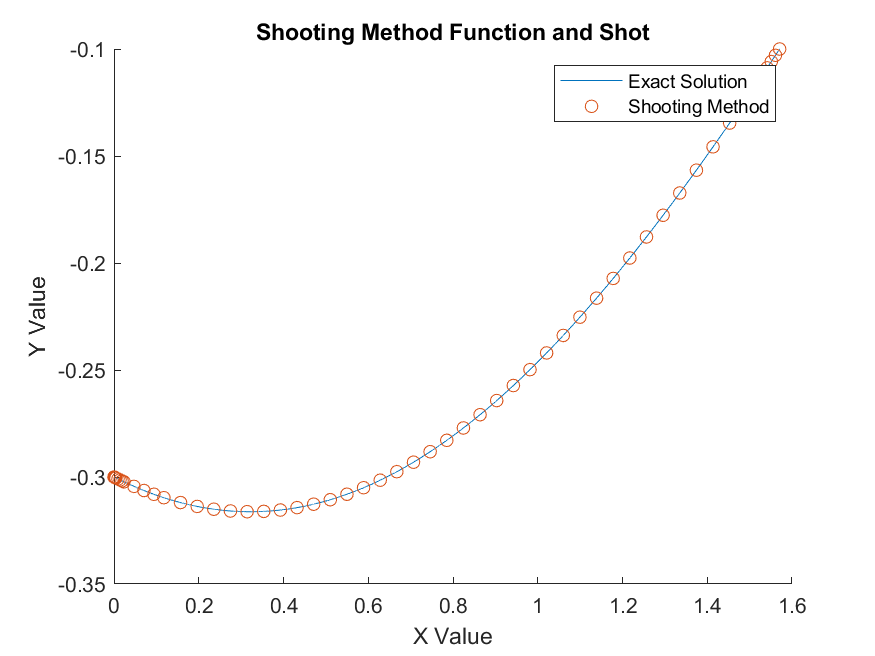
\includegraphics{./ShootingPlot1.png}
\caption{}
\end{figure}

\begin{figure}
\centering
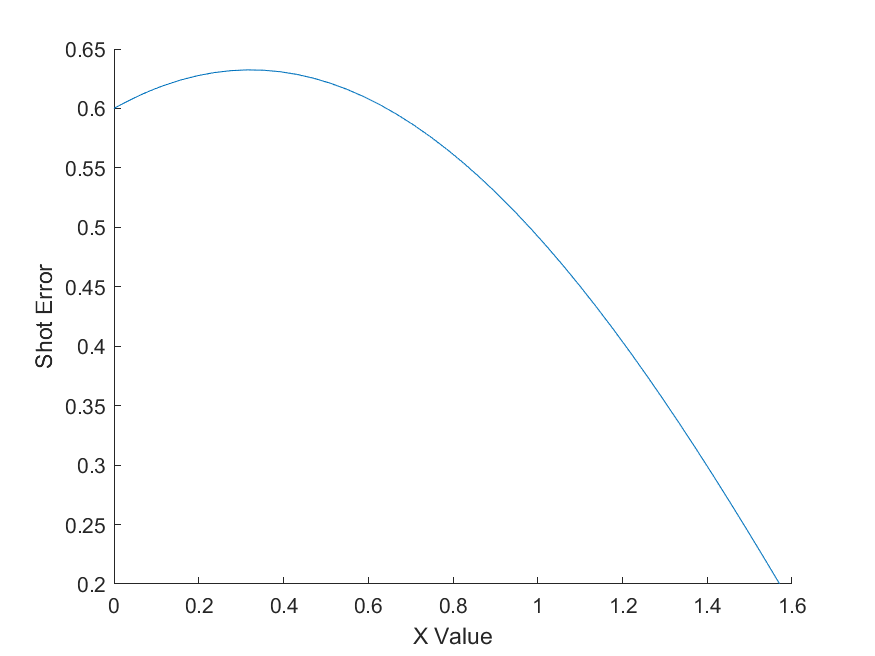
\includegraphics{./ShootingErr1.png}
\caption{}
\end{figure}

\subsection{b.}\label{b.}

Consider the two-point boundary value problem for the unknown u(x):

\[u'' = 3u - x + x^2, u(0) = 0, u(1) + u'(1) = 1\]

Explain in detail how to solve this problem with the shooting method.

Using the previous boundary value problem we compared our soluation
after using our ODE solver to the actual value of beta. Let us use that
approach again. Before beta was a single value, but now beta is
\(1 - u'(1)\). In this instance u'(1) represents our value of the first
derivative at the right endpoint.

\[\lambda y_1(b) + (1-\lambda)y_2(b) = \beta - \lambda y_1'(b) + (1-\lambda)y_2'(b)\]
\[\lambda y_1(b) + (1-\lambda)y_2(b) + \lambda y_1'(b) + (1-\lambda)y_2'(b) = \beta\]
\[\lambda (y_1(b) + y_1'(b)) + (1-\lambda)(y_2(b)+y_2'(b)) = \beta\]
\[\lambda = \frac{\beta - (y_2(b)+y_2'(b))}{(y_1(b) + y_1'(b)) - (y_2(b)+y_2'(b))}\]

With the new boundary we merely have to update the way that we find our
value of lambda to ensure that this boundary condition stays true by
incorporating the value of \(u'(b)\).

\section{Problem 2}\label{problem-2}

Consider the differential equation

\[y'' = -(y')^2 - y + ln(x), 1\leq x \leq 2\] \[y(1) = 0, y(2) = ln(2)\]

Show that the exact solution is:

\[y(x) = ln(x)\]

Implement the shooting method for this problem in Matlab. Use the Matlab
solver ode45. Note that this is a non-linear problem, so you need to use
a secant iteration. Since the secant iteration converges quickly if the
initial guess is good, it is crucial to get a good initial guess. Try
the values \(z_1 = 1, z_2 = 0.5\).

You may chooose the tolerance to be 10\^{}-9, and maximum number of
iterations for teh secant method to be 5. Plot the approximate solutions
together with the exact solution. Plot also the error.

My Script:

\begin{verbatim}
% Non-Linear boundry value shooting method

% set initial values
tol = 10^-9;
alpha = 0;
beta = log(2);
z1 = 1;
z2 = 0.5;
y = [alpha; z1; alpha; z2];
nmax = 5;

% t is in the range 0 to pi / 2
tSpan = [1 2];
[t, yOut] = ode45(@odefun,tSpan,y);

n = 0;
testVal = 100000000000000;

while abs(testVal - beta) > tol && n < nmax
    % lat row num
    lastRow = length(yOut(:,1));
    % secant iteration
    testVal = z2 + (beta - yOut(lastRow,3))*((z2 - z1)/(yOut(lastRow,3)-yOut(lastRow,1)));
    if abs(testVal - beta) < tol
        break
    end
    % update z vals;
    z1 = z2;
    z2 = testVal;
    y(2) = z1;
    y(4) = z2;
    [t, yOut] = ode45(@odefun,tSpan,y);
    n = n + 1;
end
yOutput = lambda .* yOut(:,1) + (1 - lambda) .* yOut(:,3);
disp(yOut(lastRow,1))
disp(yOut(lastRow,3))
disp(testVal)

tFunc = [tSpan(1):0.0001:tSpan(2)];
yFunc = log(tFunc);

% Plot function
figure
hold on
plot(tFunc, yFunc)
scatter(t, yOutput)
xlabel("X Value")
ylabel("Y Value")
title("Shooting Method Function and Shot")
legend("Exact Solution", "Shooting Method")

% Plot error
yFuncErr = log(t);
yFuncErr = abs(yOutput - yFuncErr);
figure
hold on
plot(t, yFuncErr)
xlabel("X Value")
ylabel("Shot Error")
title("Error")


function out=odefun(t,y)
    % system to solve
    out = zeros(4,1);
    out(1) = y(2);
    out(2) = -1 * y(2)^2 - y(1) + log(t);
    out(3) = y(4);
    out(4) = -1 * y(4)^2 - y(3) + log(t);
end
\end{verbatim}

Plot is figure 3 and error plot is figure 4.

\begin{figure}
\centering
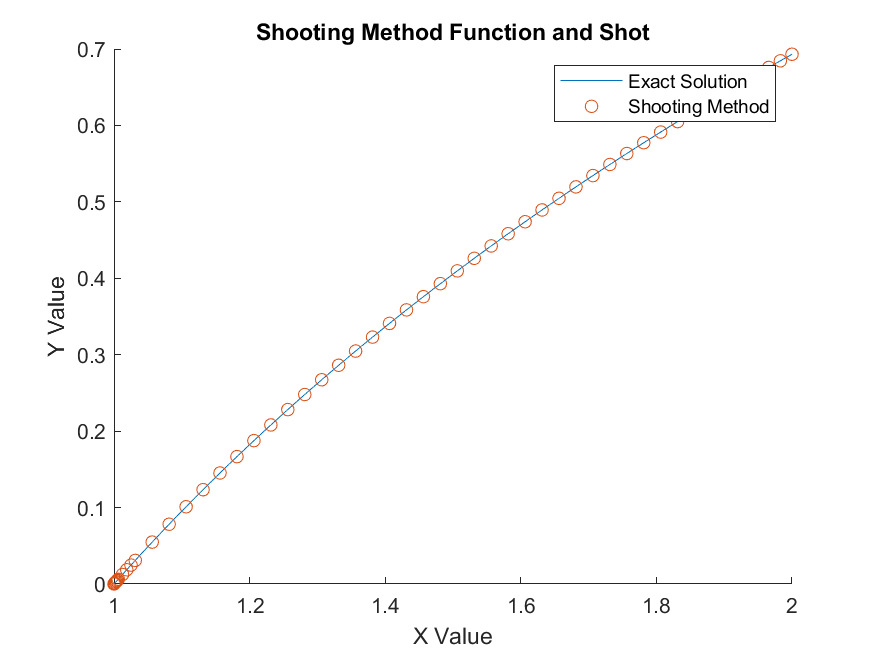
\includegraphics{./ShootingPlot2.png}
\caption{}
\end{figure}

\begin{figure}
\centering
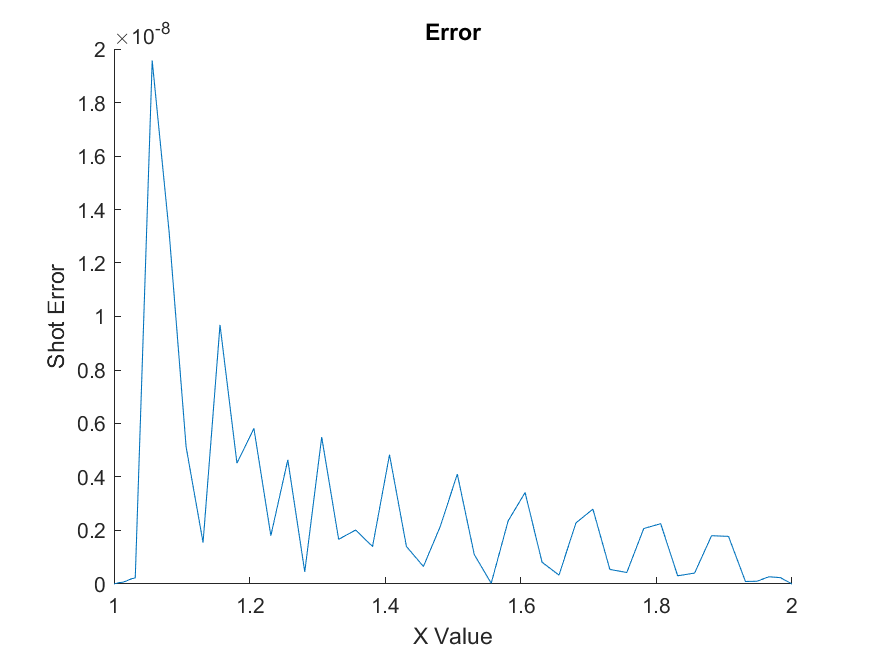
\includegraphics{./ShootingErr2.png}
\caption{}
\end{figure}

Really small error!

\section{Problem 3}\label{problem-3}

Consider the same equation as in Problem 1A. We will now compute the
approximate solutions with the finite difference method.

\[y'' = y' + 2y + cos(x); 0 \leq x \leq \frac\pi2\]
\[y(0) = -0.3, y(\frac\pi2) = -0.1\]

\subsection{a.}\label{a.-1}

Consider a uniform grid with \(h = (b - a)/N\). Set up a the finite
difference method for the problem. Write out this tridiagonal system of
linear equations for \(y_i\).

Recall the finite difference approximations:

\[y'(x_i) \approx \frac{y_{i+1} - y_{i-1}}{2h}\]
\[y''(x_i) \approx \frac{y_{i+1}-2y_i + y_{i-1}}{h^2}\]

Let's insert these equations into the ODE.

\[y'' = y' + 2y + cos(x)\]
\[\frac{y_{i+1}-2y_i + y_{i-1}}{h^2} = \frac{y_{i+1} - y_{i-1}}{2h} + 2 * y_i + cos(x_i)\]
\[\frac{y_{i+1}-2y_i + y_{i-1}}{h^2} - \frac{y_{i+1} - y_{i-1}}{2h} - 2 * y_i = cos(x_i)\]
\[y_{i+1}-2y_i + y_{i-1} - \frac{h}2(y_{i+1} - y_{i-1}) - 2h^2 * y_i = h^2cos(x_i)\]
\[ (1+\frac{h}2)y_{i-1} - 2(1+h^2) * y_i + (1-\frac{h}2)y_{i+1} = h^2cos(x_i)\]

So we have the tridiagonal matrix a with the upper diagonal
\(c_i = 1-\frac{h}2\), the lower diagonal \(a_i = 1+\frac{h}2\) and the
actual diagonal \(d_i = 2(-1 -h^2)\). The load vector b has the first
element \(b_1 = h^2cos(x_1) - a_1\alpha\) the middle elements
\(b_i = h^2cos(x_i)\) and the last element
\(b_{n-1} = h^2cos(x_{n-1})-c_{n-1}\beta\)

\subsection{b.}\label{b.-1}

Write a Matlab program that computes the approximate solution \(y_i\).
You may either use the Matlab solver to solve the linear system, or use
code for tri-diagonal systems. Test your program for N=10 and N =20.
Plot the approximate solutions together with the exact solution. Plot
also the errors.

Plot is figure 5 and error is figure 6.

\begin{figure}
\centering
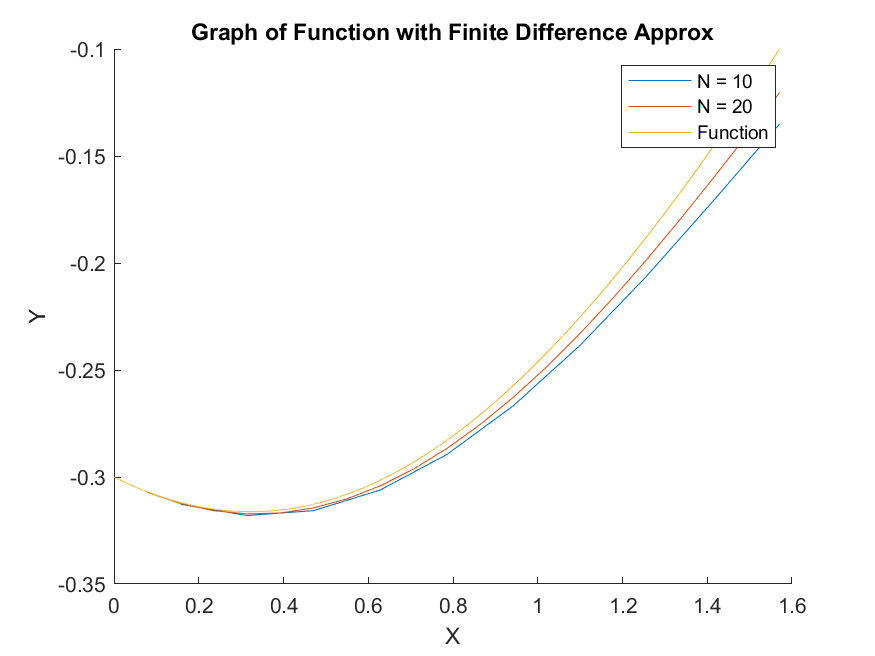
\includegraphics{./FinitePlot.png}
\caption{}
\end{figure}

\begin{figure}
\centering
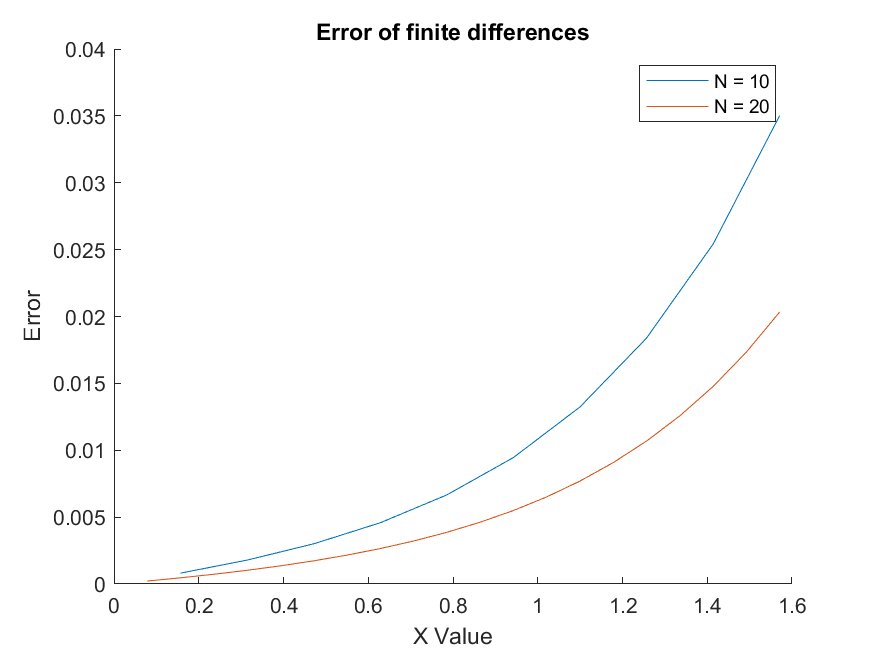
\includegraphics{./FinitErr.png}
\caption{}
\end{figure}

Script:

\begin{verbatim}
% Finite Difference Method

% Set inital values
N = [10, 20];
start = 0;
endP = pi / 2;
alpha = -0.3;
beta = -0.1;
H = (endP - start)./N;
firstErr = zeros(N(1),1);
secErr = zeros(N(2),1);
x1 = zeros(N(1),1);
x2 = zeros(N(2),1);

figure
hold on

% Calculate each
for j = 1:2
   n = N(j);
   h = H(j);
   x = zeros(n,1);
   a = zeros(n,1);
   b = zeros(n,1);
   c = zeros(n,1);
   d = zeros(n,1);
   
   A = zeros(n,n);
   
   for i = 1:n
       x(i) = start + i * h;
       a(i) = 1 + h / 2;
       c(i) = 1 - h / 2;
       d(i) = -1 * 2 * (1 + h^2);
       A(i,i) = d(i);
       if i == 1
           b(i) = h^2 * cos(x(i)) - a(i) * alpha;
           A(i, i+1) = c(i);
       elseif i == n
           b(i) = h^2 * cos(x(i)) - c(i) * beta;
           A(i, i-1) = a(i);
       else
           b(i) = h^2 * cos(x(i));
           A(i, i+1) = c(i);
           A(i, i-1) = a(i);
       end
   end
   yVals = A\b;
   yAct = -1 .* (sin(x) + 3 .* cos(x))./10;
   
   if j == 1
       firstErr = abs(yVals - yAct);
       x1 = x;
   else
       secErr = abs(yVals - yAct);
       x2 = x;
   end
   
   plot(x,yVals)
end

xF = [0:0.0001:pi/2];
y = -1 .* (sin(xF) + 3 .* cos(xF))./10;
plot(xF,y)
legend("N = 10","N = 20","Function")
xlabel("X")
ylabel("Y")
title("Graph of Function with Finite Difference Approx")

figure
hold on
plot(x1, firstErr)
plot(x2, secErr)
xlabel("X Value")
ylabel("Error")
legend("N = 10","N = 20")
title("Error of finite differences")
\end{verbatim}


\end{document}
